\documentclass{article}
\usepackage{graphicx}
\usepackage{hyperref}

\hypersetup {
	colorlinks=true,
	urlcolor=blue,
	linkcolor=black
}

\graphicspath{ {images/} }

\title{Anglers' Log}
\author{Cohen Adair}
\date{April 18th, 2016}

\begin{document}
	\maketitle
	
	\begin{abstract}
		Anglers' Log is an Android application that allows users to track, analyze, and share their catches in the sport of fishing.  It can be useful for many reasons, but most notably the ability to use past experience and data to be better prepared and have more success in future fishing trips.  Anglers' Log is a fairly large application; it includes a \textit{SQLite} back end, an organized and versatile data model, and a modern, fluid user interface (UI), all of which work without an internet connection or login from the user.  This document covers these areas in detail as well as outlines what I learned and challenges I faced throughout the development process.
	\end{abstract}
	\newpage
	
	\tableofcontents
	\newpage
	
	
	\section{Technologies}
	
	Anglers' Log is an Android application that utilizes the Android API.  Android applications are written in the Java programming language and include configuration files in JSON, user interface components in XML, as well as the use of many image resources.
	
	At first I thought Anglers' Log would be great as a web application, which it could be, but nobody carries a laptop or desktop computer with them when they fish.	What they do carry, however, is their phones.  As an avid fisherman, I thought it would be great if I could take pictures of my catches and record them to be used as a reference later.  After talking with a few other people, creating a mobile application was the clear choice.
	
	Throughout the development process I used several third party technologies including \textit{Instabug} for bugs and feedback, \textit{Crashlytics} for crash reporting, and \textit{HelloCharts} for graphing statistical data.  In situations like this I feel is it much better to utilize other, more developed solutions, than to try and create your own.  Also, implementing other peoples' code or programs is often done in the real world and I think experience in this area is an asset.
	
	There are many solutions out there that provide mobile applications the ability to report bugs and send feedback and crash reports, but \textit{Instabug} and \textit{Crashlytics}, for me, stood out.  Their free versions are more than enough for what I needed, they both had outstanding reviews, and they both had great web interfaces for managing bug reports and crashes.  I do not regret choosing either of them.
	

	\section{Architecture}
	
	Most Android applications follow an architecture similar to the one shown in Figure 1:  three or four layers that relay information to one another.  This keeps different parts of the application separate; each part has one job, and one job only.
	
	\begin{figure}[h]
		\caption{Anglers' Log Architecture}
		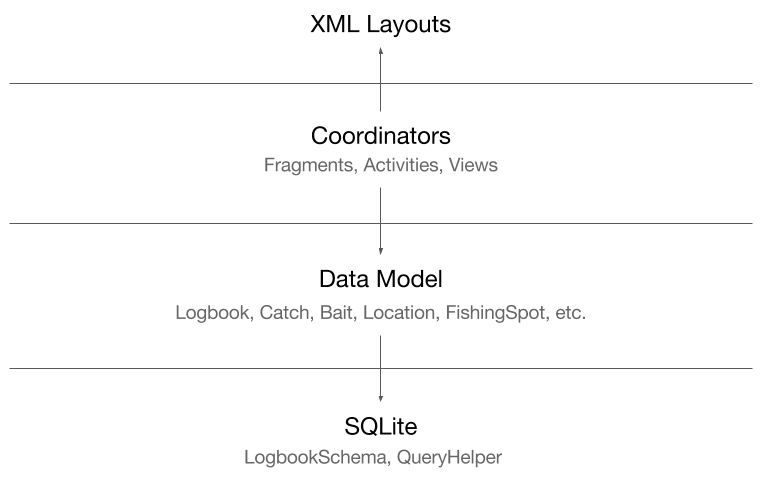
\includegraphics[width=\textwidth]{architecture}
	\end{figure}


	\subsection{XML Layouts}
	
	In Android, almost all UI elements - views, activities, fragments - have an XML component.  They provide the baseline for what the application will look like to the user.  The XML elements cannot initialize communication outside of their scope.  That is, they can only communicate with another layer if the other layer initializes the conversation.
	
	Android has two top level UI elements utilized by every application - \texttt{Fragment} and \texttt{Activity}.  Both elements can contain several child views or, in some cases, other fragments.  \texttt{Fragments} are Android's solution to reusable user interfaces.  The difference between a \texttt{Fragment} and a \texttt{View} (which is also reusable) is that a \texttt{Fragment} shares its parent \texttt{Activity}'s life cycle which includes, but is not limited to, creating, starting, and pausing the interface.

	In Anglers' Log, there is a single top-level \texttt{Activity} that houses the different pages.  Each page is a \texttt{Fragment}, and these pages are created, destroyed, moved, and even overlapped, reacting to what the user does.

	Depending on the page, Anglers' Log \texttt{Fragments} might be a parent to another \texttt{Fragment}, some \texttt{View} subclasses or a combination of both.


	\subsection{Coordinators}
	
	The coordinators manage the communication between the model and views, and if desired override the XML components.  They also define the behavior of the application.  They handle touch events, animations, and page transitions.  The coordinators are the heart of the application, and normally include subclasses of Android’s \texttt{Fragment} and \texttt{Activity} classes.
	
	At the core of Anglers' Log's UI there is a layout manager.  The layout manager is a static class that stores the different \texttt{Fragment} instances for each page.  Since all of Anglers’ Log's pages are almost identical in structure it makes sense to have a class to store this information and that can be utilized by the main \texttt{Activity} to reduce repeated code.

	All pages have a master fragment.  This is the fragment that is shown when someone taps an item in the navigation menu.  From the master fragment, the user can navigate to the detail fragment, or if they are on a tablet, the detail fragment can be updated from interaction with the master fragment. 

	Figure 2 shows a coordinating structure that keeps things organized and reduces a lot of repeated code.
	
	\begin{figure}[h]
		\caption{Anglers' Log UI Coordination System}
		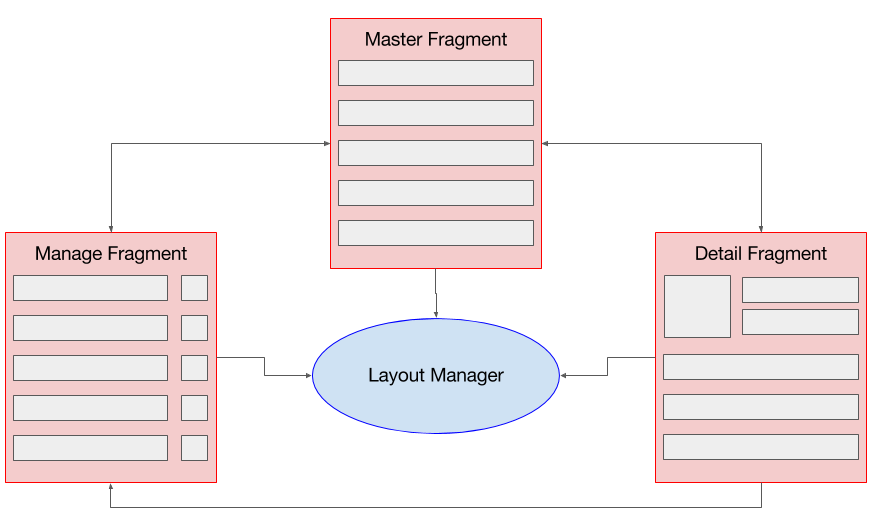
\includegraphics[width=\textwidth]{coordinators}
	\end{figure}
	
	When an application utilizes Android's navigation drawer tools, it provides a callback interface for what to do when each item in the menu is clicked.  In a lot of cases, developers use a \texttt{switch} statement or a series of \texttt{if} statements to figure out which UI element should be displayed.  Sometimes this works just fine, but when you have several elements with almost identical behavior, you find yourself repeating these statements many times throughout the code for different scenarios.

	Having a layout manager keeps all this behavior in one spot.  The layout manager provides a method to get the behavior from an input navigation item.  From this single method, all the behavior of this page is stored in an object, and this object can be read from anywhere.  It makes the code more organized, and easier to understand and maintain.


	\subsection{Data Model}
	
	The data model is the collection of Java objects that correspond to the database's schema.  In almost all cases, the model objects can be independent of the Android API.  The model's purpose is to conveniently relay information to and from the back end data storage to the application coordinators.  

	There is one singleton class in the model - \texttt{Logbook}.  The \texttt{Logbook} class gets, adds, deletes, updates, and manipulates the database.  The hard work of these processes, however, is relayed to the smaller model objects - the \texttt{Catch}, \texttt{Bait}, \texttt{Location}, \texttt{Trip} classes, for example.  All these objects can get data from the database, but in most cases the \texttt{Logbook} gets the data and uses it as input for the methods of the smaller objects.

	The smaller model objects' job is to map a single database row to a single Java object.  For example, when the \texttt{Logbook} requests all catches from the database, each row returned is mapped to a \texttt{Catch} object and an array of \texttt{Catch} objects is returned from the \texttt{Logbook} method.

	The advantage to this structure is, again, to keep things organized.  Working with the coordinators to properly display data to the user should not interfere with \textit{SQLite} and vise versa. Keeping these processes separate makes the development process much smoother.
	

	\subsection{SQLite}
	
	The recommended method of data storage for Android is \textit{SQLite} because it is small and very fast.  Android provides excellent tools for interacting with a \textit{SQLite} database in code, including tutorials on how to implement \textit{SQLite} data to Java object mapping.

	Each Anglers' Log model object has an \texttt{id} property.  An \texttt{id} is a string of 24 randomly generated characters.  Once an object is created and is assigned an \texttt{id}, and the \texttt{id} never changes.  This \texttt{id} is passed around from the database to the model to the coordinators so that when the object associated with that \texttt{id} is displayed to the user it is the most up to date version.
	
	This is done because in Anglers' Log, users can modify these objects as they wish.  If they changed a \texttt{Bait} name, it would not be good if the wrong name was displayed to the user.
	

	\section{Image Cache}
	
	The images stored by Anglers' Log are fairly large in size, and are not often viewed by the user at their full size.  There are thumbnail versions of these images used all over the application such as to show in a gallery or in a list item.

	Unless told otherwise, Android automatically scales the source of an \texttt{ImageView} to correctly fit inside the view.  If all the developer wants to do is load one or two images this method works just fine, but when they want to implement a gallery or some other scrolling view that includes scrolling images they run into a big problem.  Android cannot keep up with the image-to-\texttt{ImageView} scaling and the user interface lags tremendously.  

	The easiest way to solve this problem is to scale the images in a background thread,, but it is inefficient to repeatedly scale these to the same size - it wastes time and RAM.  Caching these scaled thumbnails ensures no unnecessary scaling is done; it also greatly increases the speed at which the thumbnails are seen by the user in the future.
	
	\begin{figure}[h]
		\caption{Anglers' Log Image Cache/Resizing}
		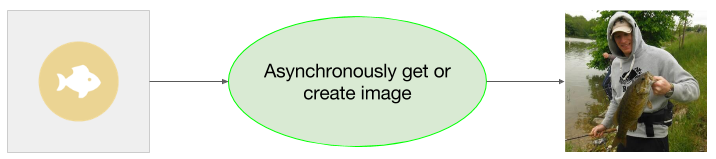
\includegraphics[width=\textwidth]{imagecache}
	\end{figure}

	Figure 3 shows this process as seen by the user.  An \texttt{ImageView} is given the source of a place holder image, and a request for the actual image is sent to the image cache.  The image cache will then check to see if this image (in the correct size) is in memory.  If it is not, it will check the disk cache, and if it still does not exist it will scale the original image, save it to disk and place it in the memory cache.  Finally, the thumbnail image is sent back to the \texttt{ImageView} to be displayed to the user.

	Anglers' Log will still run without a system like this, but it will lag very badly and will likely push users to an alternative solution.
	

	\section{Backup}

	There are many backup solutions available for Android, but none were viable for both data and image storage.	A server costs too much money, and Android's automatic backup service would only work for a handful of images, not the hundreds stored by users.
		
	Anglers' Log takes the \textit{SQLite} data, exports it as JSON, and packs it, along with the user's images, into a \texttt{.zip} archive, and is then shipped to a cloud storage solution selected by the user.

	This method is not automatic for the user, but the steps are very simple.  A user exports Anglers' Log data locally on their device or to a cloud storage solution they have on their device.  Once the data is exported, it can be imported from another device that has Anglers' Log already installed.  This new device can be run by either Android or iOS.

	The implementation is very simple.  Each model object has its own \texttt{toJson()} method that returns a single JSON object representation of that instance.  This is done for all model object instances until all \texttt{Logbook} properties are included in a single JSON object.  This final object is then converted to a \texttt{String}, written to a file, and added to the exporting archive.

	Having each model separated keeps things very organized and reduces the risk of error because each object only has to worry about itself.  As long as it does its job correctly, the final result will also be done correctly.
	

	\section{Challenges}
	
	No project comes without challenges.  Most of mine were small details that resulted in unexpected behavior.  These did not end up being a lot of trouble after some research.  There is also the obvious challenge of learning new things and a new API, but thanks to Google's excellent documentation that part was not too painful.

	There is one challenge I want to mention, though, and it is not about overcoming a challenging programming problem, it is keeping your code readable and maintainable.  I think this is often overlooked when it is such an important part of development.  It may seem like an easy thing to do, but in large projects, especially those on your own, it is easy to forget, and just throw in some undocumented code that seems to work without thinking about whether or not it is the best or even correct solution.

	After a few months of development I had a lot of code, and I am obviously not going to remember all of it.  Looking back at that code it was a lot of the time difficult to understand why I did something, or even how it worked.  As you can imaging this was incredibly frustrating.  This is when I realized I needed to take the time to properly document and organize my code.  Ever since, making updates has been much, much easier.
	
	
	\section{Conclusion}
	
	Overall, I am very happy with how Anglers' Log turned out.  It took a lot of work and a lot of dedication.  I learned a lot, not only about Android development, but new programming techniques, object oriented design, databases, and the software develop-test-release life cycle.

	Even if Anglers' Log is not used by many people it is a tool I love and something I will use for a very long time.
	
	\newpage
	 
	 \section{Credits}
	 
	 \begin{description}
	 	\item[Instabug] is a method for mobile application users to file bug reports or provide feedback to developers.
	 	
	 	\url{https://instabug.com/} 
	 	 
	 	\item[Crashlytics] is a method for developers to receive crash logs from users.  No work is required from the user; \textit{Crashlytics} runs completely in the background.
	 	
	 	\url{https://try.crashlytics.com/}
	 	
	 	\item[Hello Charts] is an extensive charting tool for Android.  I use it for pie charts to show statistical data based on a user's catch history.
	 	
	 	\url{https://github.com/lecho/hellocharts-android}
	 	
	 	\item[Subsampling Scale Image View] is a modified \texttt{ImageView} that allows users to zoom in and out using the familiar pinch zoom and double tap methods.  I use this solution in the Anglers' Log gallery.
	 	
	 	\url{https://github.com/davemorrissey/subsampling-scale-image-view}
	 	
	 	\item[Android Random Color] is a simple utility for generating a random color from a few parameters.  I use this in combination with \textit{Hello Charts} to generate unique colors for the pie chart.
	 	
	 	\url{https://github.com/lzyzsd/AndroidRandomColor}
	 	
	 	\item[Circle Image View] is an \texttt{ImageView} subclass that provides rounded corners.  I use this for almost all thumbnails throughout Anglers' Log.
	 	
	 	\url{https://github.com/hdodenhof/CircleImageView}
	 	
	 \end{description}
	 
\end{document}